\vspace{-2em}
\section{Number Base System Encodings}

\label{sec:base_encodings}
 
\noindent
We now explore how to represent our base two or any other base number in a fixed-length encoding.

% \begin{Def}[Turing Machine]

%     A \textbf{Turing Machine} is a theoretical computational model used to describe the capabilities of a general-purpose \textbf{computer}. It consists of an infinite tape (memory) and a read/write head processing symbols on the tape, one at a time, according to a set of predefined rules. The machine moves left or right, reading or writing symbols, and changing states based on what it reads. 
    
%     The machine \textbf{halts} once it reaches a final state or continues indefinitely. Serving as a flexible, \textbf{higher-order function} (a function which receives functions).
% \end{Def}

\begin{Def}[Number Base Fixed-length Encoding]

    \label{def:number_base_fixed_length_encoding}

    \noindent
    Each memory cell in the computers stack is an integer value represented in a fixed base, typically \(B = 2\), 
    meaning \textbf{binary}. Where each digit is less than the base \(B\). We represent integers in memory as:

    \[
    a = \sum_{i=0}^{k-1} a_i B^i
    \]
    
    \noindent
    Where \( a_i \) represents the individual digits, and \(B\) is the base. For large integers, computations may require manipulating several memory cells to store the full number.
\end{Def}

\noindent
\begin{Example}[Binary \& Decimal Representations] 

Consider the integer, $a = 13$, in base, $B := 2$ \textbf{(binary)}, using Definition \ref{def:number_base_fixed_length_encoding}:

\Large
\[
a = \underbracket{(\text{\textcolor{red}{1}} \cdot 2^3) + (\text{\textcolor{red}{1}} \cdot 2^2) + (\text{\textcolor{red}{0}} \cdot 2^1) + (\text{\textcolor{red}{1}} \cdot 2^0)}_{\text{binary: \textcolor{red}{1101}}} = 8 + 4 + 0 + 1 = 13
\]
\normalsize

\vspace{1em}
\noindent
Here, the coefficients $a_3 = 1$, $a_2 = 1$, $a_1 = 0$, and $a_0 = 1$ correspond to the binary digits of $13$, where each 
power of $2$ represents the binary place value. Similarly, if we want to represent, $a = 45$, in base, \textbf{$B := 10$ (decimal)}:

\[
a = 4 \cdot 10^1 + 5 \cdot 10^0 = 40 + 5 = 45
\]

\noindent
In this case, the coefficients $a_1 = 4$ and $a_0 = 5$ correspond to the decimal digits of $45$.
\end{Example}

\noindent
We continue to common bases that one may encounter in computing and mathematics:
\begin{Def}[Hexadecimal]
    \textbf{Hexadecimal} base $B=16$, using digits 0-9 and the letters A-F, where:
    \begin{center}
        $A=10$, $B=11$, $C=12$, $D=13$, $E=14$, and $F=15$.
    \end{center} Hexadecimal is commonly used in computing due to its compact representation of binary data. E.g., 
    A \underline{\textbf{byte} (8 bits)} can be represented as two hexadecimal digits, simplifying the display of binary data.
\end{Def}

\newpage

\begin{theo}[Base $2\leftrightarrow16$ Conversion]

    Let bases \( B:=2 \) (binary) and \( H:=16 \) (hexadecimal). At a high-level:

    \vspace{.5em}
    
    \noindent \textbf{Binary to Hexadecimal:}
    \begin{enumerate}
        \item Group $B$ digits in sets of 4, right to left. \textbf{Pad} leftmost group with 0's if necessary for a full group.
        \item Compute each group, replacing the result with their $H$ digit.
        \item Finally, combine each $H$ group.
    \end{enumerate}
    
    \noindent \textbf{Hexadecimal to Binary:}
    \begin{enumerate}
        \item Convert each $H$ digit into a 4 bit $B$ group.
        \item Finally, combine all $B$ groups.
    \end{enumerate}
    \noindent
    Additionally, we may also trim any leading 0's.
\end{theo}

\noindent
\begin{Example}[Base $2\leftrightarrow16$ Conversion]
    \begin{itemize}
        \item Binary to Hexadecimal:
        \[
        101101111010_2 \quad \Rightarrow \quad \text{Group as } (\underbracket{[1011]}_{11} \ \underbracket{[0111]}_{7} \ \underbracket{[1010]}_{10}) \quad \Rightarrow \quad B7A_{16}
        \]
        \item Hexadecimal to Binary:
        \[
        3F5_{16} \quad \Rightarrow \quad [0011]\ [1111]\ [0101]_2 \Rightarrow \quad 1111110101_2
        \]
        \noindent
    \end{itemize}

\end{Example}

\noindent
The following definition is for completeness: applications of such a base are currently seldom.
\begin{Def}[Unary]
    
    \textbf{Unary}, base $B=1$. A system where each number is represented by a sequence of the same symbol. 
    This system is more theoretical than practical given today's systems.\\

    \noindent
    Given a toy unary system, we may represent numbers with a single symbol ``I'': $5 = \texttt{IIIII}$ or $2= \texttt{II}$. 
    The absence of symbols may represent 0.
\end{Def}

\begin{Def}[Most \& Least Significant Bit]
    
    In a binary number, the \textbf{most significant bit (MSB)} is the leftmost bit. The \textbf{least significant bit (LSB)} is the rightmost bit.\\

    \noindent
    E.g., In the byte (8 bits), $[1111 \ 1110]_2$, the MSB = 1 and the LSB = 0.
\end{Def}

\begin{theo}[Adding Binary]

    We may use the add and carry method alike decimal addition:\\

    \begin{minipage}{0.30\textwidth}
        \begin{itemize}
            \item $0 + 0 = 0$
            \item $0 + 1 = 1$
        \end{itemize}
    \end{minipage}
    \hfill
    \begin{minipage}{0.58\textwidth}
        \begin{itemize}
            \item $1 + 0 = 1$
            \item $1 + 1 = 0 \quad (\text{add 1 to the next digit (left)})$
        \end{itemize}
    \end{minipage}

    \vspace{1em}
    \noindent
    We call the last step a \textbf{carry}, as we carry our overflow to the next digit.
\end{theo}

\begin{Example}[Binary Addition]
    
\noindent   
Adding $0010\ 0011\ 0100_2$ and $0100_2$:
    \begin{equation*}
        \begin{array}{B3}
             1       &                             1000 &  \carry 0\textcolor{red}{1}00 \\
              {} + 0 &                             0001 &  0\textcolor{red}{1}00 \\ \hline
                   1 &                             1001 &  1000 \\
        \end{array}
        \end{equation*}
\noindent
Where $[1\ 1000\ 0100]_2 + [0\ 0001\ 0100]_2 = [1\ 1001\ 1000]_2$.
\end{Example}

\begin{Def}[Signed Binary Numbers - Two's Complement]
    
    In a \textbf{two's complement system}, an $n$-bit signed (positive or negative) binary number can represent values in the range $[-2^{n-1}, 2^{n-1}-1]$. Then by most significant bit (MSB):
    \begin{itemize}
        \item If MSB is 0, the number is positive;
        \item If MSB is 1, the number is negative.
    \end{itemize}
    \noindent
    \textbf{Conversion to Two's Complement :}
    \begin{enumerate}
        \item Take an unsigned binary number and invert all bits, turning 0's to 1's and 1's to 0's.
        \item Finally add 1 to the least significant bit.
    \end{enumerate}
\end{Def}

\begin{Example}[Two's Complement Conversion]
    
    \noindent
    Converting $-5$ into a 4-bit two's complement:
    \begin{align*}
        5 \rightarrow 0101 \quad & \text{(binary for 5)} \\
         1010 \quad & \text{(inverted)} \\
         1011 \quad & \text{(add 1)}
    \end{align*}
    Thus, $-5$ is represented as $1011$ in 4-bits under two's complement.
\end{Example}

\begin{Def}[Big \& Little Endian]
    
    \textbf{Big Endian} and \textbf{Little Endian} are two ways of storing multi-byte data in memory:
    \begin{itemize}
        \item \textbf{Big Endian:} The most significant byte (MSB) is stored at the lowest memory address 
        (How English reads and writes).
        \item \textbf{Little Endian:} The least significant byte (LSB) is stored at the lowest memory address.
    \end{itemize}

    \noindent
    Subsequent bytes are stored in increasing order. \textbf{Note:} A single byte has no endianness.
\end{Def}

\begin{figure}[ht!]
    \centering
    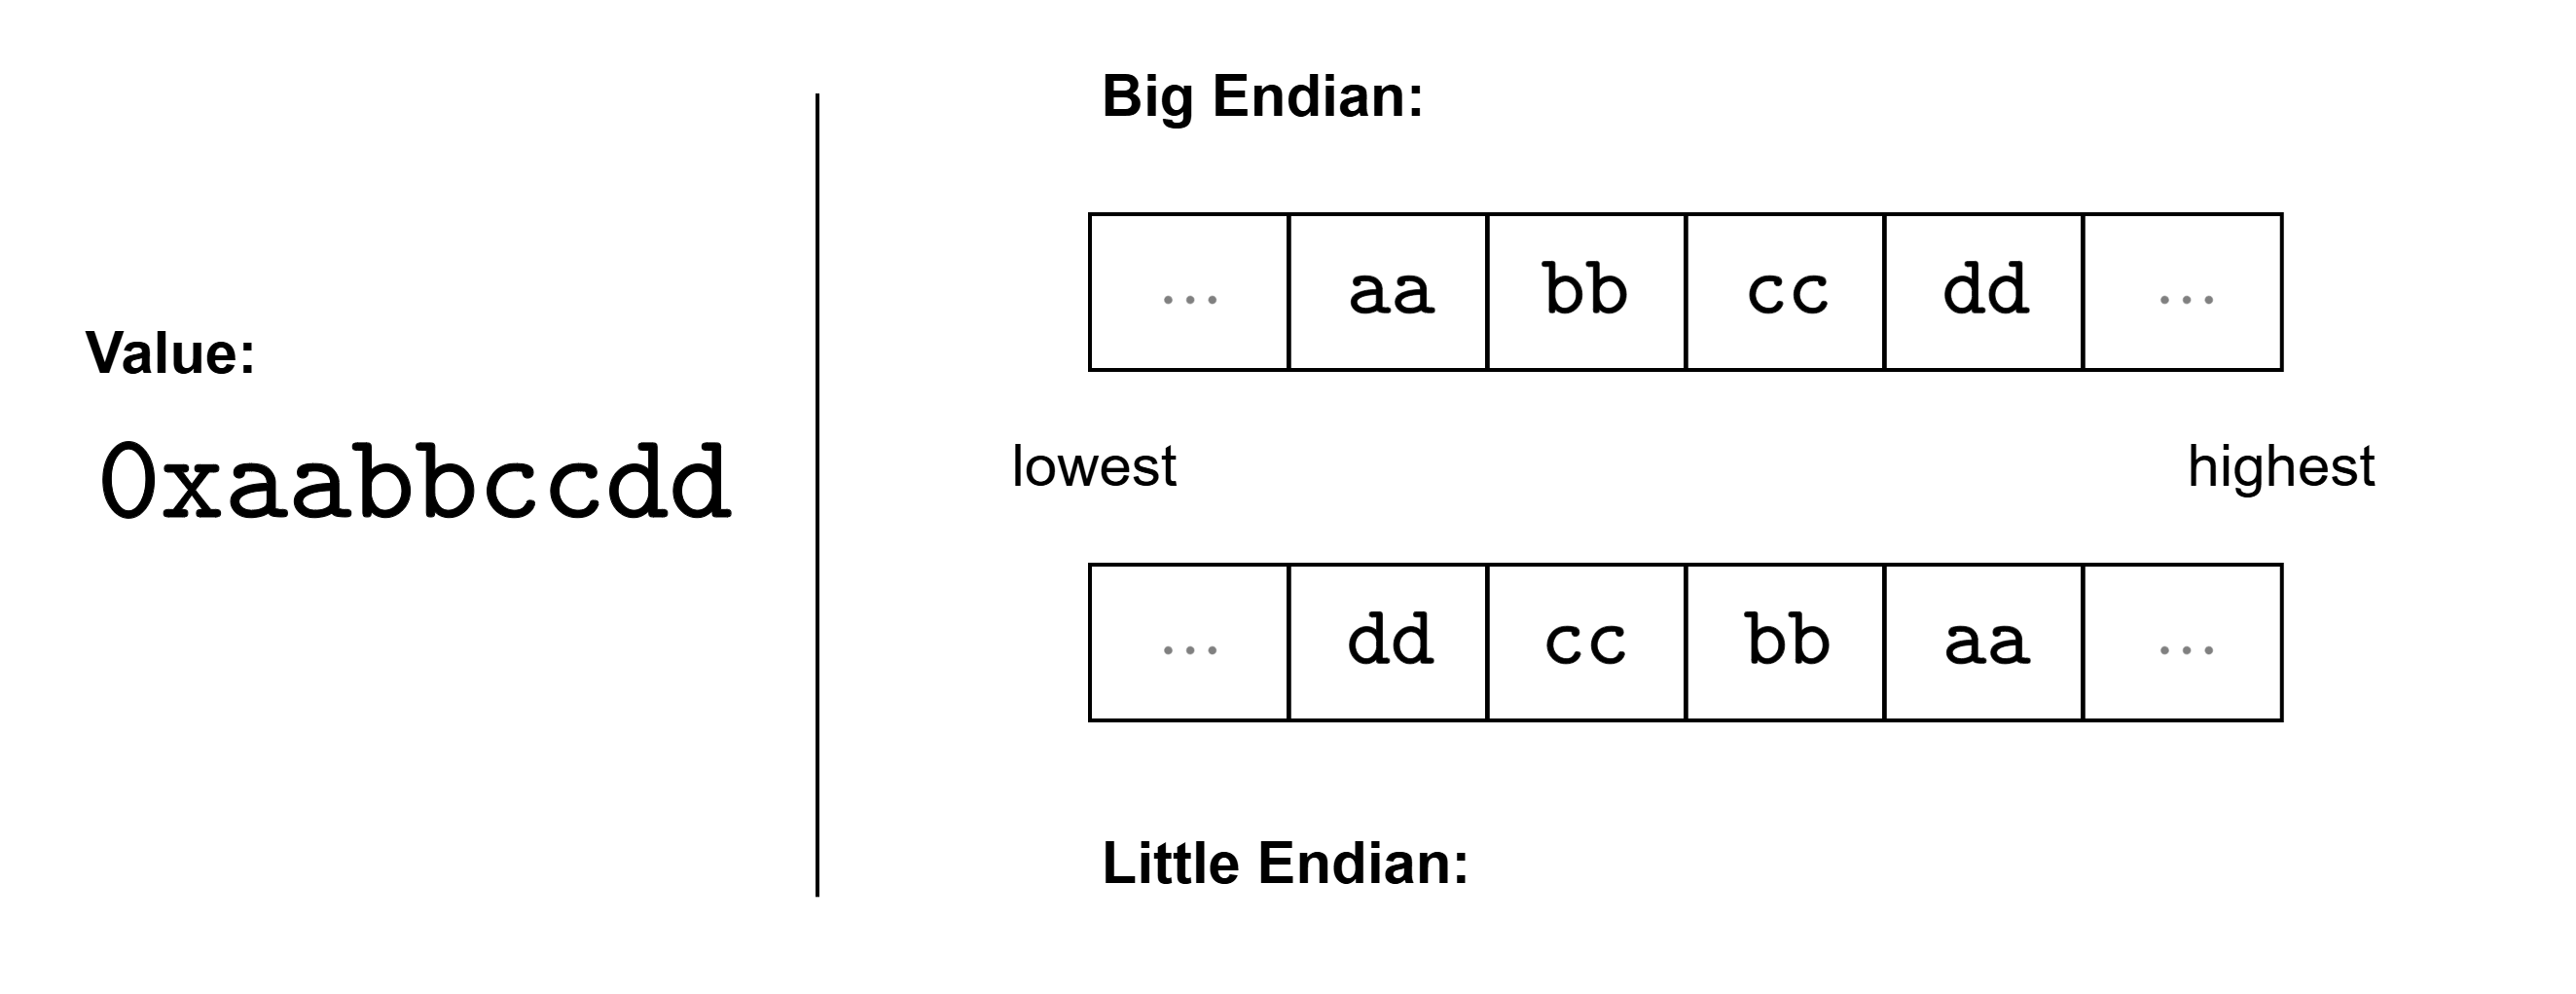
\includegraphics[width=0.8\textwidth]{sections/comp/big_endian.png}
    \caption{Big Endian vs Little Endian Representation of $0xaabbccdd$. Recall that $0x$ denotes a hexadecimal number,
    and $aa$ is a whole byte (8 bits) in hexadecimal.}
\end{figure}

\begin{Tip} The name ``endian'' comes from \emph{Gulliver's Travels} by Jonathan Swift, where
    Gulliver encounters two factions of people while traveling to the island of Lilliput. 
    One faction, the \textbf{Big-Endian}, believes that eggs should be cracked at the big end, 
    while the other faction, the \textbf{Little-Endian}, believes that eggs should be cracked at the little end.
\end{Tip}

    
\newpage

\begin{theo}[Commincation \& Endianess]

    \label{theo:communication_endianess}

    When communicating between systems, it is crucial to agree on the endianness of the data being sent. 
    If one system uses big-endian and the other uses little-endian, the data will be misinterpreted. 
    E.g., According to \href{https://datatracker.ietf.org/doc/html/rfc793}{RFC 793}, all the fields in network 
    headers must be big-endian.\\

    \noindent
    \rule{\textwidth}{0.4pt}\\
    \noindent
    \textbf{Note:} When debugging one might encounter an issue with endianness. Suppose we read the little-endian value
    $0xaabbccdd$ two bytes at a time. This gives us $A_1 = 0xccdd$ and $A_2 = 0xaabb$. The computer read both values 
    $B_1 = ddcc$ and $B_2 = bbaa$, translating it before sending it back to the debugger. This can cause issues as this is far beyond 
    the original value.
\end{theo}